\section{Analysis}
\label{sec:analysis}

\subsection{Per-Operator Local/Global Split}
\label{sec:operator_split}

Figure~\ref{fig:operator_gradient} decomposes TaxEI's recovery performance by operator (seed=42, $N{=}11$--$12$ tasks per operator). The results reveal a binary split rather than a smooth gradient:

\begin{itemize}[nosep,leftmargin=*]
\item \textbf{Local operators}: C4 (observation masking) shows $+9.1$pp improvement over Vanilla; P1 (step order swap) shows $0.0$pp change.
\item \textbf{Global operators}: Both C1 (context truncation, $-8.3$pp) and P2 (sub-goal deletion, $-8.3$pp) degrade performance.
\end{itemize}

\begin{figure}[t]
\centering
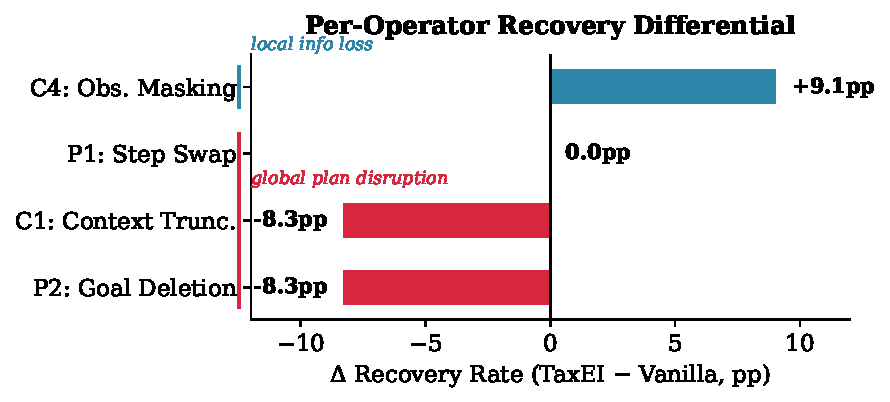
\includegraphics[width=\columnwidth]{figures/paper/fig2_operator_gradient.pdf}
\caption{Per-operator recovery delta (TaxEI $-$ Vanilla, seed=42). Local/observable errors (C4, P1) are neutral-to-beneficial; global/cascading errors (C1, P2) are harmful. $N{=}11$--$12$ per operator; differences of $\pm1$ task correspond to $\pm$8--9pp. Exploratory analysis.}
\label{fig:operator_gradient}
\end{figure}

This split aligns with an intuitive distinction: local errors (a masked observation, a swapped step) leave the plan's causal structure intact, allowing the model to learn recovery patterns. Global errors (truncated context, deleted sub-goals) propagate downstream, making all subsequent actions unreliable---the model memorizes noise rather than learning recovery.

C1 (context truncation) is classified as a Context-type operator but behaves like a global operator: truncating the context window forces all subsequent decisions to rely on incomplete history, functionally equivalent to a cascading plan disruption.

We emphasize that these per-operator results are exploratory: at $N{=}11$--$12$ tasks per operator, each $\pm1$ task flip corresponds to $\pm$8--9pp, and we cannot draw statistically robust conclusions from single-task margins.

\subsection{Training-Evaluation Paradox}
\label{sec:paradox}

At $\geq$25\% injection, models achieve \emph{lower} training loss but \emph{worse} evaluation performance. TaxEI-50\% reaches a final loss of 0.259 (vs.\ Vanilla 0.288) yet evaluates at 51.1\% (vs.\ 61.7\%). This paradox does not hold at 10\% injection, where training loss (0.308) remains above Vanilla---the model has not yet begun memorizing injected patterns at sub-threshold doses.

This pattern is consistent with findings on memorization in noisy-label settings: models first learn clean patterns, then memorize noise \cite{arpit2017memorization}. In our setting, injected error trajectories are well-formed sequences that the model can memorize as surface patterns \cite{zhou2023lima}, improving training metrics without generalizing to unseen tasks.
